\subsection{TA Grading Page (Nick)}

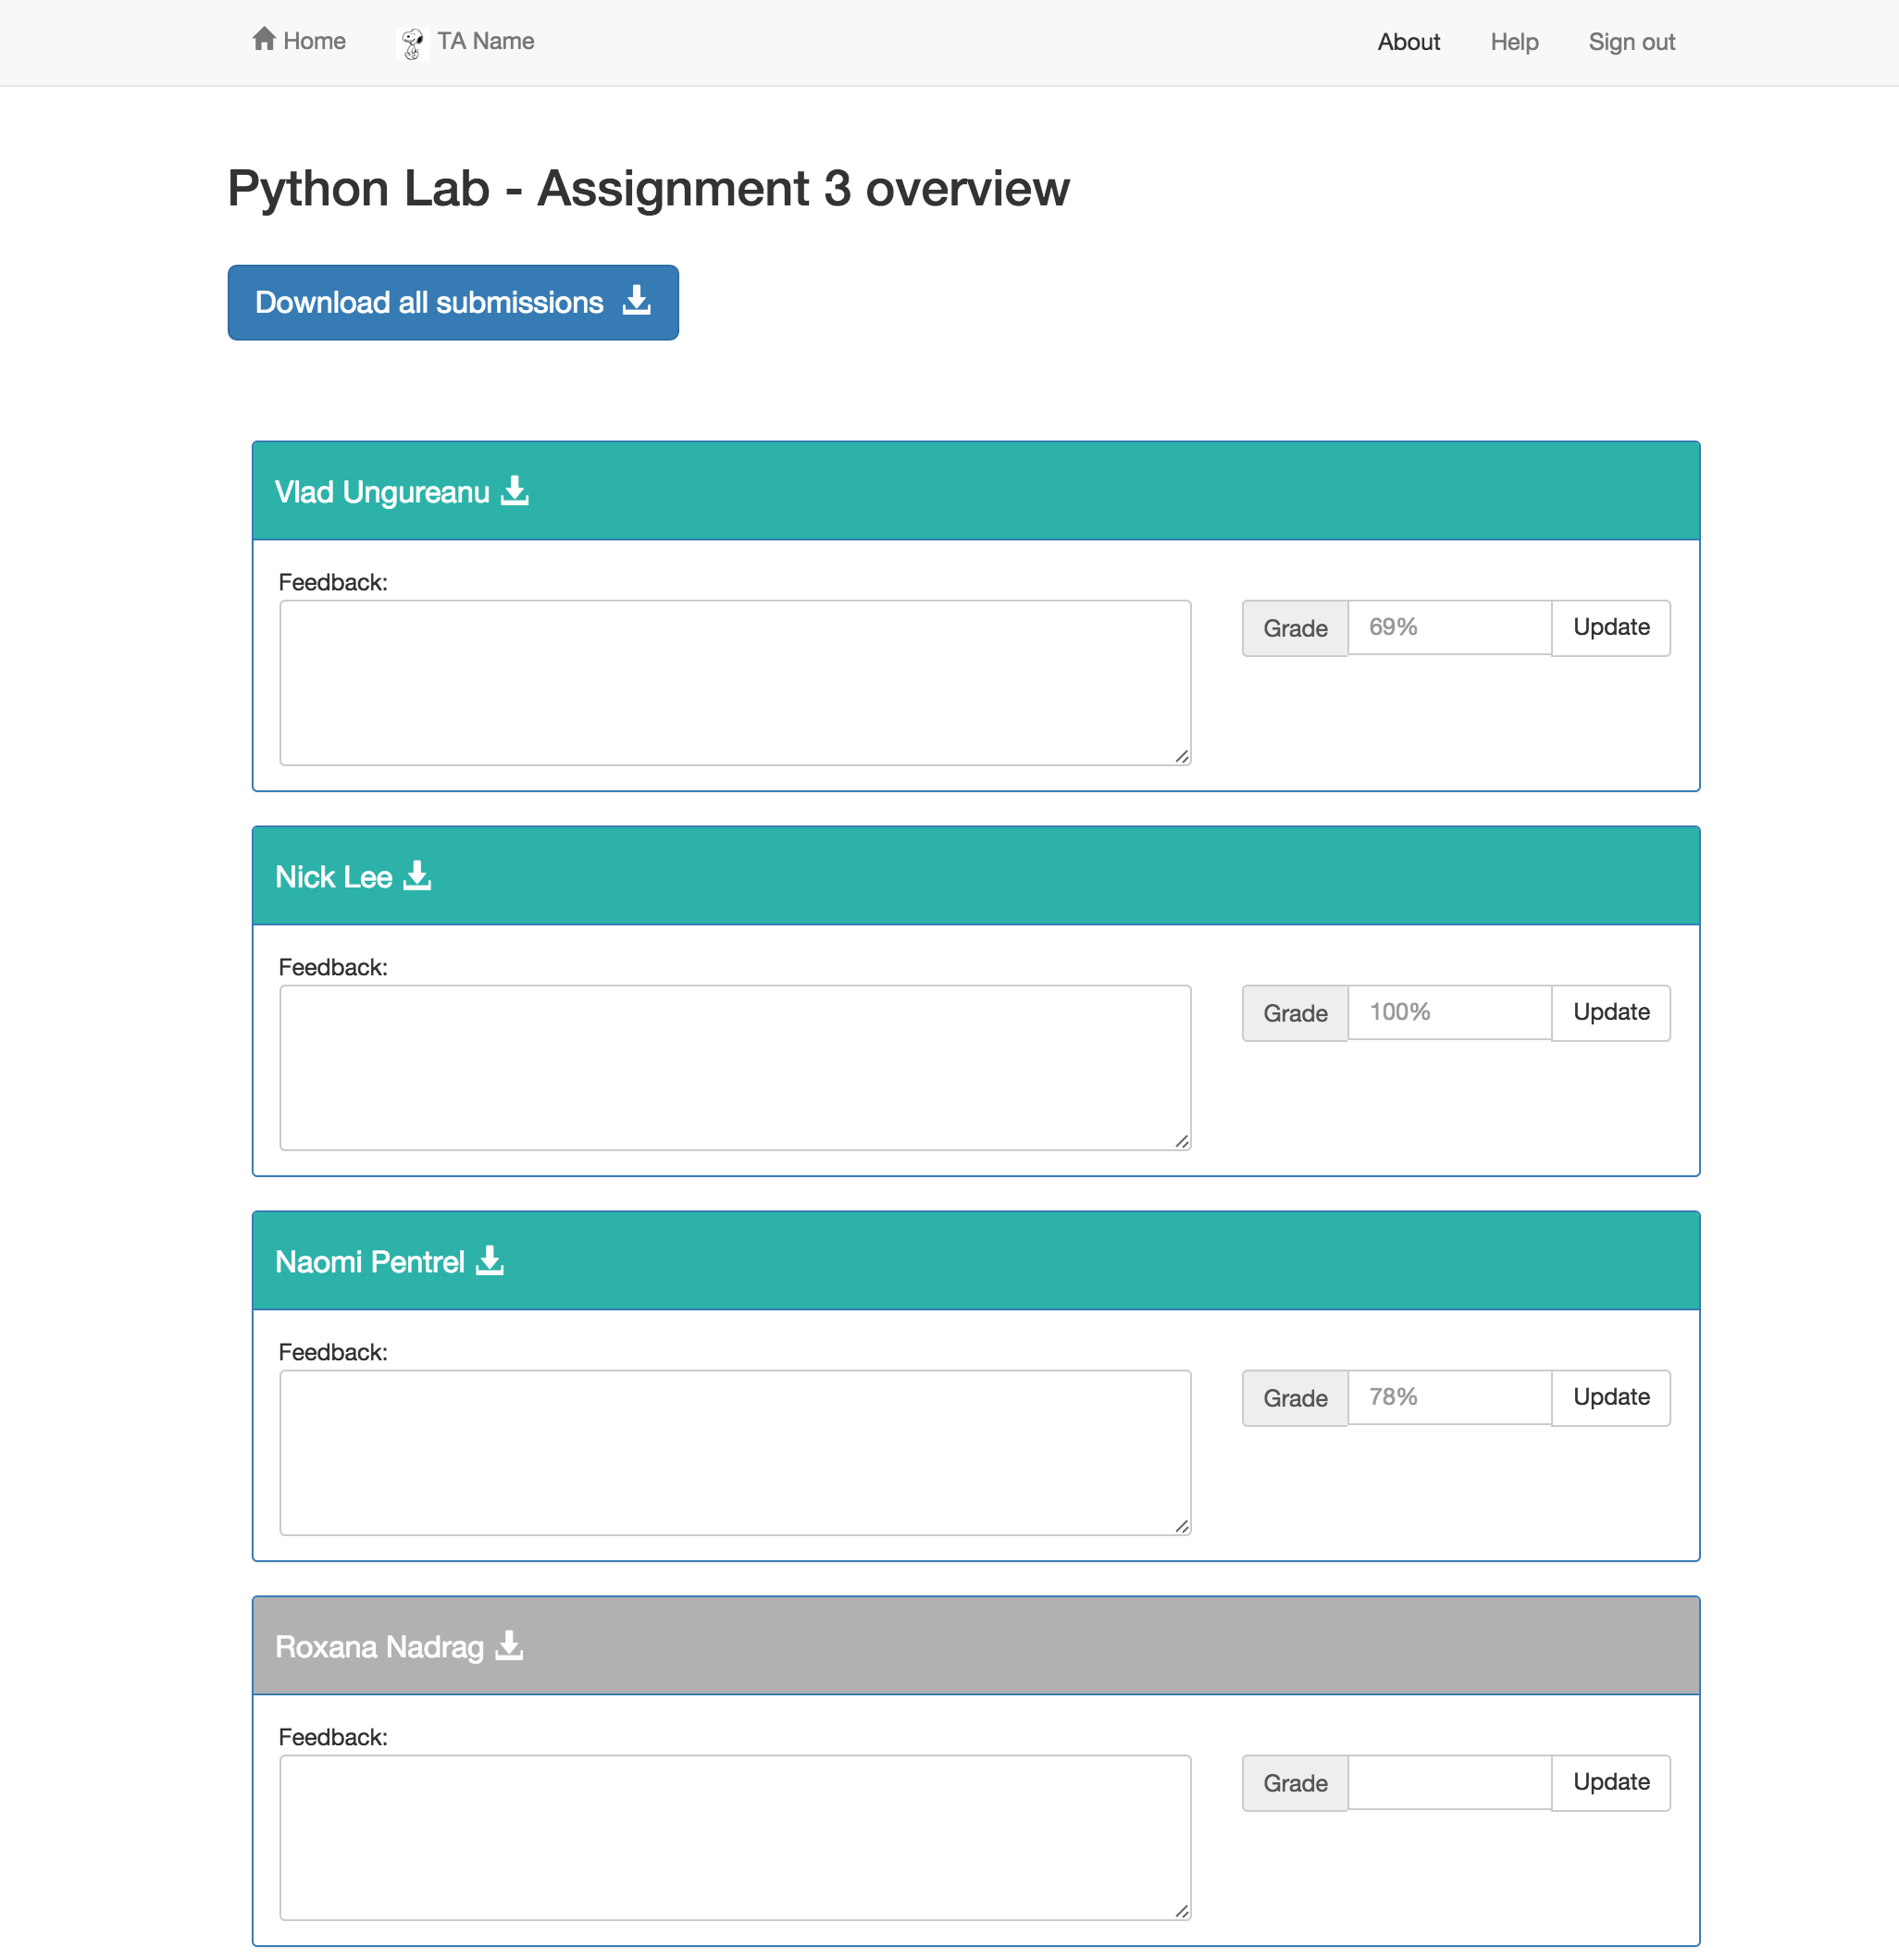
\includegraphics[width=\textwidth]{screenshots/GradingAssignmentOverview.png}

Each assignment grading page follows the same layout, with the page content being centred to help the user focus. A simple heading communicates what assignment is being graded, two batch jobs can be run from a well-known location (always the top of the page), and the remainder of the page is simply a list of submissions in need of grading. 

No default field is initially focused; this is because the TA must first download the submissions. Tabbing through the page with the keyboard will always follow the order "Feedback, Grade, Submit" in order to minimise the amount of steps involved with grade entry, which is important for grading large numbers of small assignments. We placed the comment box before the grade box in order to encourage TAs to provide comments for grades; when tabbing through the page, the comment field will be selected first, which makes it tougher to skip.

All submission boxes are colour-coded, such that a graded assignment is aqua, an ungraded assignment is orange, and an empty submission is grey. Ungraded submissions are not omitted because it is sometimes necessary for assignments to be submitted via alternate methods such as paper or email. While the purpose of a grey field is slightly different from what it was on the overview page (non-actionable), most blank submissions will never receive a grade other than zero, and so they can be considered non-actionable for the most part. 

Ample space is provided between assignment entries in order to reduce the chance of visual confusion. In a complete implementation, JavaScript would also be used to turn the currently selected region's background to a light grey in order to further differentiate what's being edited. Avoiding a pure grid layout also helps in creating a more comfortable view for the user.

Different sizes between the comment and grade fields provide further visual differentiation, and the larger size of the feedback box implies its significance. In many programming labs, the feedback is more important than the grade.  
